% This is text associated with the open textbook "Open Electromagnetics"
% See immediately below for author, date
% This work is licensed under the Creative Commons Attribution-ShareAlike 4.0 International License. (CC BY-SA 4.0) 
% To view a copy of the license, visit http://creativecommons.org/licenses/by-sa/4.0/

%ORB TITLE Radiation Pattern
%ORB AUTHOR 0        # S.W. Ellingson, Virginia Tech (ellingson@vt.edu)
%ORB DATE 20191212   # yyyymmdd
%ORB ABSTRACT 

\label{m0205_Radiation_Pattern} % <-- Must match name of this file and module directory name.  Don't mess with this!
\index{pattern (radiation)|(}
\index{polarization|(}

The \emph{radiation pattern} of a transmitting antenna describes the magnitude and polarization of the field radiated by the antenna as a function of angle relative to the antenna.  A pattern may also be defined for a receiving antenna, however, we defer discussion of the receive case to a later section. 

The concept of radiation pattern is closely related to the concepts of directivity and gain (Section~\ref{m0203_Directivity_and_Gain}). 
The principal distinction is the explicit consideration of polarization.
In many applications, the polarization of the field radiated by a transmit antenna is as important as the power density radiated by the antenna.
For example, a radio communication link consists of an antenna which is transmitting separated by some distance from an antenna which is receiving.  
Directivity determines the power density delivered to the receive antenna, but the receive antenna must be co-polarized with the arriving wave in order to capture all of this power.  

The radiation pattern concept is perhaps best explained by example.
The simplest antenna encountered in common practice is the electrically-short dipole (ESD), which consists of a straight wire of length $L$ that is much less than one-half of a wavelength.
In Section~\ref{m0198_Radiation_from_an_Electrically-Short_Dipole}, it is shown that the field radiated by an ESD which is located at the origin and aligned along the $z$-axis is:
%
\begin{equation}
\widetilde{\bf E}({\bf r}) \approx  \hat{\bf \theta} j \eta \frac{I_0\cdot\beta L}{8\pi} ~\left(\sin\theta\right) ~\frac{e^{-j\beta r}}{r}
\label{m0205_eESDE}
\end{equation}
%
where $I_0$ represents the magnitude and phase of the current applied to the terminals, $\eta$ is the wave impedance of the medium, and $\beta=2\pi/\lambda$ is the phase propagation constant of the medium.
Note that the reference direction of the electric field is in the $\hat{\bf \theta}$ direction; therefore, a receiver must be $\hat{\bf \theta}$-polarized relative to the transmitter's coordinate system in order to capture all available power.
A receiver which is not fully $\hat{\bf \theta}$-polarized will capture less power.
In the extreme, a receiver which is $\hat{\bf \phi}$-polarized with respect to the transmitter's coordinate system will capture zero power.
Thus, for the $\hat{\bf z}$-oriented ESD, we refer to the $\hat{\bf \theta}$-polarization of the transmitted field as ``co-polarized'' or simply ``co-pol,'' and
the $\hat{\bf \phi}$-polarization of the transmitted field as ``cross-pol.''

At this point, the reader may wonder what purpose is served by defining cross polarization, since the definition given above seems to suggest that cross-pol should always be zero.
In common engineering practice, cross-pol is non-zero when co-pol is different from the \emph{intended} or \emph{nominal} polarization of the field radiated by the antenna.
In the case of the ESD, we observe that the electric field is always $\hat{\bf \theta}$-polarized, and therefore we consider that to be the nominal polarization.  Since the actual polarization of the ESD in the example is precisely the same as the nominal polarization of the ESD, the cross-pol of the ideal ESD is zero.  
If, on the other hand, we arbitrarily define $\hat{\bf \theta}$ to be the nominal polarization and apply this definition to a different antenna that does not produce a uniformly $\hat{\bf \theta}$-polarized electric field, then we observe non-zero cross-pol.
Cross-pol is similarly used to quantify effects due to errors in position or orientation,  or due to undesired modification of the field due to materials (e.g., feed or mounting structures) near the transmit antenna.
Summarizing: 
%
%%%%%%%%%%%%%%%%%%%%%%%%%%%%%%%%%%%%%%%%%%%%%%%
%ORB HIGHLIGHT
\begin{mdframed}[backgroundcolor=yellow!20,nobreak=true] 
\emph{Co-pol} is commonly defined to be the intended or nominal polarization for a particular application, which is not necessarily the actual polarization radiated by the antenna under consideration. \emph{Cross-pol} measures polarization in the orthogonal plane; i.e., deviation from the presumed co-pol.
\end{mdframed}
%%%%%%%%%%%%%%%%%%%%%%%%%%%%%%%%%%%%%%%%%%%%%%%

Returning to the ESD:  Since $\widetilde{\bf E}({\bf r})$ depends only on $\theta$ and not $\phi$, the co-pol pattern is the same in any plane that contains the $z$ axis.  
We refer to any such plane as the \emph{E-plane}.
\index{E-plane}
In general:
%
%%%%%%%%%%%%%%%%%%%%%%%%%%%%%%%%%%%%%%%%%%%%%%%
%ORB HIGHLIGHT
\begin{mdframed}[backgroundcolor=yellow!20,nobreak=true] 
The \emph{E-plane} is any plane in which the nominal or intended vector $\widetilde{\bf E}$ lies.
\end{mdframed}
%%%%%%%%%%%%%%%%%%%%%%%%%%%%%%%%%%%%%%%%%%%%%%%
%
Since the ESD is $\hat{\bf \theta}$-polarized, the E-plane pattern of the ESD is simply: 
%
\begin{equation}
\left|\widetilde{\bf E}({\bf r})\right| \approx  \eta \frac{I_0\cdot\beta L}{8\pi} ~\left(\sin\theta\right) ~\frac{1}{r}
\label{m0205_eEESD}
\end{equation}
%
This pattern is shown in Figure~\ref{m0205_fEplaneMag}.
%
\begin{figure} % <--- "[b!]" for first figure in section *only*; delete for 2nd and subsequent figures
\begin{center}
\pdftooltip{{  % note double braces
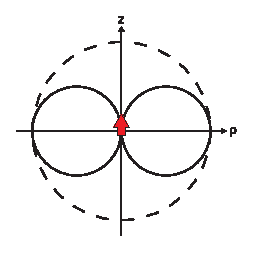
\includegraphics[width=2.5in]{modules/m0205_fEplaneMag.eps} 
% https://commons.wikimedia.org/wiki/File:Magnitude_of_the_Radiated_Field.svg
}}{A rho-z coordinate system has a dashed circle centered at the origin. Two smaller, solid line circles are centered on the rho axis. Each small circle has one edge at the origin and a second edge on the dashed circle. A red arrow pointing up rests on the origin.}
\end{center}
\centerline{\scriptsize 
\copyright~\hyperref[m0205_fEplaneMag_Credit]{S.\ Lally} 
\href{https://creativecommons.org/licenses/by-sa/4.0/}{CC BY-SA 4.0} 
} % \centerline 
\caption{
\label{m0205_fEplaneMag}
E-plane co-pol pattern for the $\hat{\bf z}$-oriented ESD.  In the unnormalized pattern scaling, the dashed circle indicates the maximum value of Equation~\ref{m0205_eEESD}.
}
\end{figure}

Equation~\ref{m0205_eEESD} is referred to as an \emph{unnormalized} pattern. 
The associated normalized pattern is addressed later in this section. 

Similarly, we define the \emph{H-plane} as follows:
\index{H-plane}
%
%%%%%%%%%%%%%%%%%%%%%%%%%%%%%%%%%%%%%%%%%%%%%%%
%ORB HIGHLIGHT
\begin{mdframed}[backgroundcolor=yellow!20,nobreak=true] 
The \emph{H-plane} is any plane in which the nominal or intended vector $\widetilde{\bf H}$ lies, and so is perpendicular to both the E-plane and the direction of propagation.
\end{mdframed}
%%%%%%%%%%%%%%%%%%%%%%%%%%%%%%%%%%%%%%%%%%%%%%%
%
In the case of the ESD, the one and only H-plane is the $z=0$ plane.
The H-plane pattern is shown in Figure~\ref{m0205_fHplaneMag}.
%
\begin{figure} % <--- "[b!]" for first figure in section *only*; delete for 2nd and subsequent figures
\begin{center}
\pdftooltip{{  % note double braces
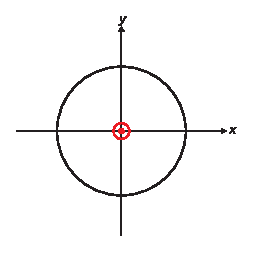
\includegraphics[width=2.5in]{modules/m0205_fHplaneMag.eps} 
% https://commons.wikimedia.org/wiki/File:FHplaneMag.svg
}}{An x-y coordinate system with a circle centered around the origin. A red “out-of-page” symbol at the origin. }
\end{center}
\centerline{\scriptsize 
\copyright~\hyperref[m0205_fHplaneMag_Credit]{S.\ Lally} 
\href{https://creativecommons.org/licenses/by-sa/4.0/}{CC BY-SA 4.0} 
} % \centerline 
\caption{
\label{m0205_fHplaneMag}
H-plane co-pol pattern for the $\hat{\bf z}$-oriented ESD. In the unnormalized pattern scaling, the radius of the circle is the maximum value of Equation~\ref{m0205_eEESD}.
}
\end{figure}

It is often useful to normalize the pattern, meaning that we scale the pattern so that its maximum magnitude corresponds to a convenient value.
There are two common scalings.
One common scaling sets the maximum value of the pattern equal to 1, and is therefore independent of source magnitude and distance.
This is referred to as the \emph{normalized pattern}.
\index{pattern (radiation)!normalized}
The normalized co-pol pattern can be defined as follows:
%
\begin{equation}
F(\theta,\phi) \triangleq \frac{\left|\hat{\bf e}\cdot\widetilde{\bf E}({\bf r})\right|}{\left|\hat{\bf e}\cdot\widetilde{\bf E}({\bf r})\right|_{max}}
\label{m0205_eNormPat}
\end{equation}
%
where $\hat{\bf e}$ is the co-pol reference direction, and the denominator is the maximum value of the electric field at distance $r$.
%
%%%%%%%%%%%%%%%%%%%%%%%%%%%%%%%%%%%%%%%%%%%%%%%
%ORB HIGHLIGHT
\begin{mdframed}[backgroundcolor=yellow!20,nobreak=true] 
A \emph{normalized pattern} is scaled to a maximum magnitude of 1, using the definition expressed in Equation~\ref{m0205_eNormPat}.
\end{mdframed}
%%%%%%%%%%%%%%%%%%%%%%%%%%%%%%%%%%%%%%%%%%%%%%%
%
Note that the value of $r$ is irrelevant, since numerator and denominator both scale with $r$ in the same way.
Thus, the normalized pattern, like directivity, does not change with distance from the antenna.

For the ESD,  $\hat{\bf e}=\hat{\bf \theta}$, so the normalized co-pol pattern is:
%
\begin{equation}
F(\theta,\phi) = \frac{\left|\hat{\bf \theta}\cdot\widetilde{\bf E}({\bf r})\right|}{\left|\hat{\bf \theta}\cdot\widetilde{\bf E}({\bf r})\right|_{max}} ~~~ \mbox{(ESD)}
\end{equation}
%
which yields simply
%
\begin{equation}
F(\theta,\phi) \approx \sin\theta ~~~ \mbox{(ESD)}
\end{equation}
%
Thus, the E-plane normalized co-pol pattern of the ESD is Figure~\ref{m0205_fEplaneMag} where the radius of the maximum value circle is equal to 1, which is 0~dB.
Similarly, the H-plane normalized co-pol pattern of the ESD is Figure~\ref{m0205_fHplaneMag} where the radius of the circle is equal to 1 (0~dB).

The other common scaling for patterns sets the maximum value equal to maximum directivity.
Directivity is proportional to power density, which is proportional to $\left|\widetilde{\bf E}({\bf r})\right|^2$.
Therefore, this ``directivity normalized'' pattern can be expressed as:
%
\begin{equation}
D_{max}\left|F(\theta,\phi)\right|^2 
\end{equation}
%
where $D_{max}$ is the directivity in whichever direction it is maximum.
For the ESD considered previously, $D_{max}=1.5$ (Section~\ref{m0203_Directivity_and_Gain}).
Therefore, the co-pol pattern of the ESD using this particular scaling is
%
\begin{equation}
1.5 \sin^2\theta ~~~ \mbox{(ESD)}
\end{equation}
%
Thus, the E-plane co-pol pattern of the ESD using this scaling is similar to Figure~\ref{m0205_fEplaneMag}, except that it is squared in magnitude and the radius of the maximum value circle is equal to 1.5, which is 1.76~dB.
The H-plane co-pol pattern of the ESD, using this scaling, is Figure~\ref{m0205_fHplaneMag} where the radius of the circle is equal to 1.5 (1.76~dB).

{\bf Pattern lobes.} Nearly all antennas in common use exhibit directivity that is greater than that of the ESD.
The patterns of these antennas subsequently exhibit more complex structure.
Figure~\ref{m0205_Sidelobes} shows an example.
%
\begin{figure} % <--- "[b!]" for first figure in section *only*; delete for 2nd and subsequent figures
\begin{center}
\pdftooltip{{  % note double braces
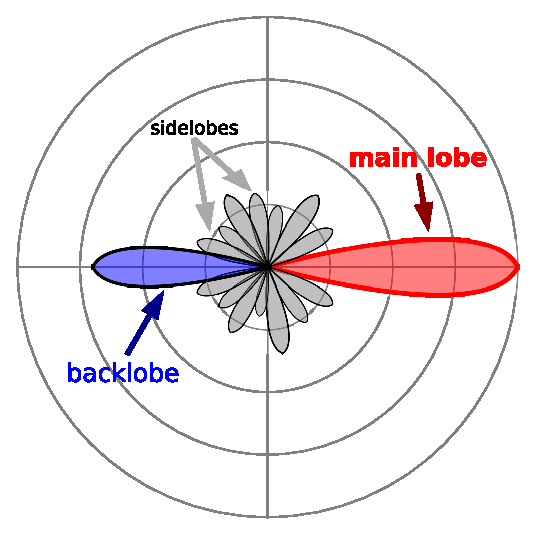
\includegraphics[width=2.5in]{modules/m0205_Sidelobes_en.eps} 
% https://en.wikipedia.org/wiki/File:Sidelobes_en.svg
}}{Flower-like pattern at the center of 4 concentric circles. The largest petal, labeled main lobe, extends on the right all the way to the outermost circle. The second largest petal, labeled backlobe, extends in the opposite direction to almost three quarters the distance covered by the main lobe. The rest of the petals, labeled sidelobes, are of varying lengths that don’t extend much farther than the innermost circle.
}
\end{center}
\centerline{\scriptsize 
\copyright~\hyperref[m0205_Sidelobes_Credit]{T.\ Truckle} 
\href{https://creativecommons.org/licenses/by-sa/4.0/}{CC BY-SA 4.0} 
(modified) 
} % \centerline 
\caption{
\label{m0205_Sidelobes}
Co-pol pattern typical of a highly directional antenna, such as a yagi. 
\index{antenna!yagi}
\index{yagi|see{antenna}}
}
\end{figure}
%
The region around the direction of maximum directivity is referred to as the \emph{main lobe}.
The main lobe is bounded on each side by a \emph{null}, where the magnitude reaches a local minimum, perhaps zero. 
Many antennas also exhibit a lobe in the opposite direction, known as a \emph{backlobe}. 
(Many other antennas exhibit a null in this direction.)
Lobes between the main lobe and the backlobe are referred to as \emph{sidelobes}.
Other commonly-used pattern metrics include \emph{first sidelobe level}, which is the ratio of the maximum magnitude of the sidelobe closest to the main lobe to that of the main lobe; and \emph{front-to-back ratio}, which is the ratio of the maximum magnitude of the backlobe to that of the main lobe.

When the main lobe is narrow, it is common to characterize the pattern in terms of \emph{half-power beamwidth} (HPBW).
\index{half-power beamwidth (HPBW)}
This is shown in Figure~\ref{m0205_HGApat}.
%
\begin{figure} % <--- "[b!]" for first figure in section *only*; delete for 2nd and subsequent figures
\begin{center}
\pdftooltip{{  % note double braces
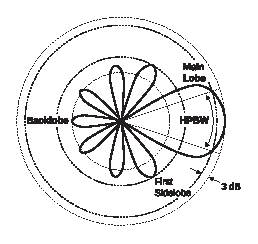
\includegraphics[width=2.5in]{modules/m0205_HGApat.eps} 
% https://commons.wikimedia.org/wiki/File:Half-Power_Beamwidth.svg
}}{Flower-like pattern sitting at the center of 4 concentric circles, not evenly spaced. The largest petal, labeled main lobe, extends on the right all the way to the outermost circle. The main lobe is labeled HPBW. The distance between the outermost circle and the circle just within it is 3 decibels.
}
\end{center}
\centerline{\scriptsize 
\copyright~\hyperref[m0205_HGApat_Credit]{S.\ Lally} 
\href{https://creativecommons.org/licenses/by-sa/4.0/}{CC BY-SA 4.0} 
} % \centerline 
\caption{
\label{m0205_HGApat}
Half-power beamwidth (HPBW).
}
\end{figure}
%
HPBW is the width of the main lobe measured between two points at which the directivity is one-half its maximum value.
As a pattern metric, HPBW depends on the plane in which it is measured.
In particular, HPBW may be different in the E- and H-planes. 
For example, the E-plane HPBW of the ESD is found to be $90^{\circ}$, whereas the H-plane HPBW is undefined since the pattern is constant in the H-plane.

{\bf Omnidirectional and isotropic antennas.}
The ESD is an example of an \emph{omnidirectional} 
\index{omnidirectional}
antenna.  An omnidirectional antenna is an antenna whose pattern magnitude is nominally constant in a plane containing the maximum directivity.  For the ESD, this plane is the H-plane, so the ESD is said to be omnidirectional in the H-plane.
The term ``omnidirectional'' does \emph{not} indicate constant pattern in all directions.
(In fact, note that the ESD exhibits pattern nulls in two directions.)
%
%%%%%%%%%%%%%%%%%%%%%%%%%%%%%%%%%%%%%%%%%%%%%%%
%ORB HIGHLIGHT
\begin{mdframed}[backgroundcolor=yellow!20,nobreak=true] 
An \emph{omnidirectional} antenna, such as the ESD, exhibits constant and nominally maximum directivity in one plane.
\end{mdframed}
%%%%%%%%%%%%%%%%%%%%%%%%%%%%%%%%%%%%%%%%%%%%%%%

An antenna whose pattern is uniform in all directions is said to be \emph{isotropic}.
\index{isotropic}
No physically-realizable antenna is isotropic; in fact, the ESD is about as close as one can get.
Nevertheless, the ``isotropic antenna'' concept is useful as a standard against which other antennas can be quantified.
Since the pattern of an isotropic antenna is constant with direction, the power density radiated by such an antenna in any direction is equal to the power density averaged over all directions.  Thus, the directivity of an isotropic antenna is exactly 1.  The directivity of any other antenna may be expressed in units of ``dBi,'' which is simply dB relative to that of an isotropic antenna.  For example, the maximum directivity of the ESD is 1.5, which is $10\log_{10}\left(1.5/1\right)$ $=$ 1.76~dBi.
Summarizing:
%
%%%%%%%%%%%%%%%%%%%%%%%%%%%%%%%%%%%%%%%%%%%%%%%
%ORB HIGHLIGHT
\begin{mdframed}[backgroundcolor=yellow!20,nobreak=true] 
An \emph{isotropic} antenna exhibits constant directivity in every direction.
Such an antenna is not physically-realizable, but is nevertheless useful as a baseline for describing other antennas.
\end{mdframed}
%%%%%%%%%%%%%%%%%%%%%%%%%%%%%%%%%%%%%%%%%%%%%%%

%%%%%%%%%%%%%%%%%%%%%

{\bf Additional Reading:}
\begin{itemize}
\item ``\href{https://en.wikipedia.org/wiki/Radiation_pattern}{Radiation pattern}''  on Wikipedia.
\end{itemize}

%%%%%%%%%%%%%%%%%%%%%%

\index{polarization|)}
\index{pattern (radiation)|)}

